\documentclass{article}
\usepackage{pdfpages}
\usepackage{graphicx}
\usepackage{listings}
\usepackage{float}
\begin{document}
\title{Modelos y Optimizaci\'on I\\ \large{Trabajo pr\'actico: An\'alisis de sensibilidad}}
\author{de Valais, Ezequiel (94463)\and Rozanec, Matias (97404)}
\date{Noviembre 2017}
\maketitle
\newpage
% FIN PRESENTACION

% Consigna
%\part{Consigna}
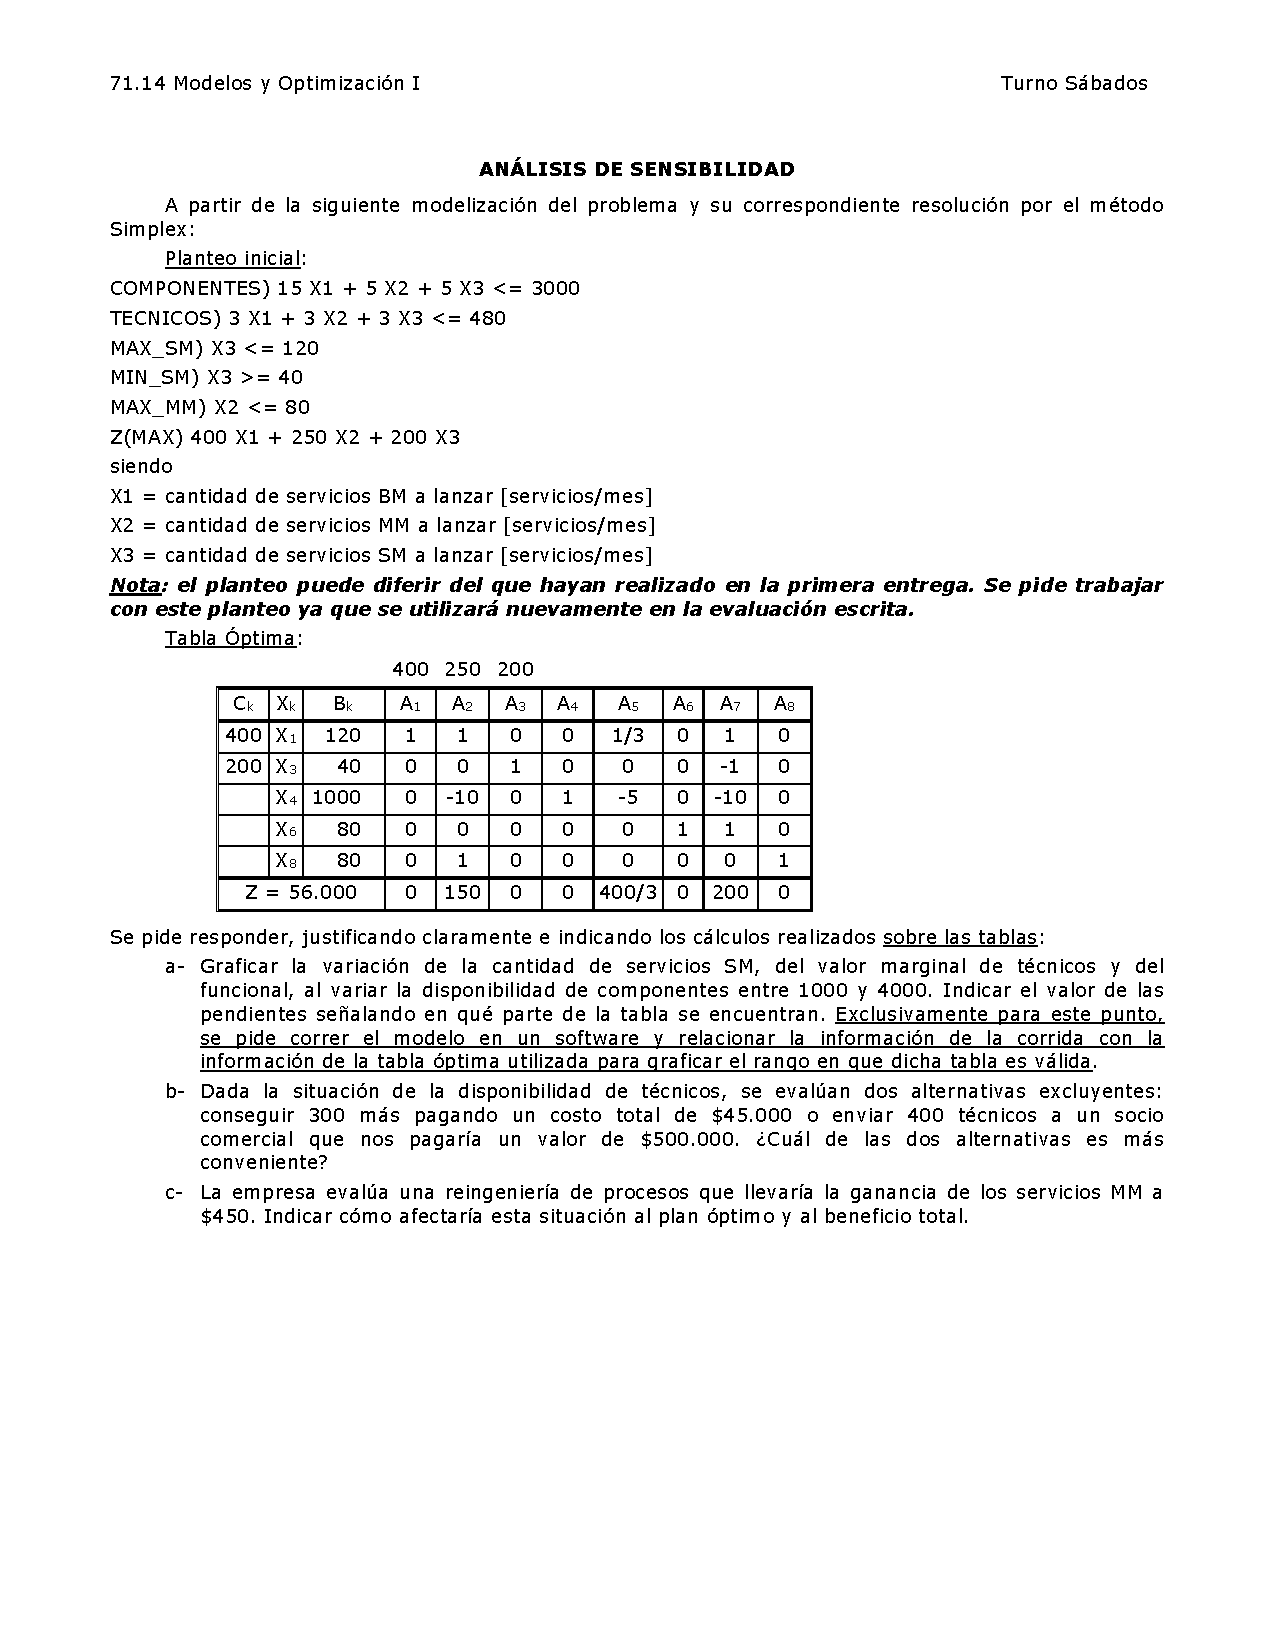
\includepdf{enunciado_analisis_sensibilidad.pdf}
\newpage

% Resolucion
\begin{enumerate}
	\item Relaci\'on entre variables del primal y del dual:\\
		\begin{tabular}{c c c}
			X1 & - & Y6 \\
			X2 & - & Y7 \\
			X3 & - & Y8 \\
			X4 & - & Y1 \\
			X5 & - & Y2 \\
			X6 & - & Y3 \\
			X7 & - & Y4 \\
			X8 & - & Y5 \\
		\end{tabular}
		\\
		Tabla \'optima del dual:\\
		\begin{tabular}{|c  c  c | c  c  c  c  c  c  c  c | c |}
			\hline
			 \multicolumn{3}{|c|}{} & 3000 & 480 & 120 & -40 & 80 & & &\\ \hline
			 Ck & Yk & Bk & A1 & A2 & A3 & A4 & A5 & A6 & A7 & A8\\ \hline 
			 480 & Y2 & 400/3 & 5 & 1 & 0 & 0 & 0 & -1/3 & 0 & 0\\
			 -40 & Y4 & 200 & 10 & 0 & -1 & 1 & 0 & -1 & 0 & 1\\
			 0 & Y7 & 150 & 10 & 0 & 0 & 0 & -1 & -1 & 1 & 0\\ \hline
			 \multicolumn{3}{|c|}{Z=56000} & -1000 & 0 & -80 & 0 & -80 & -120 & 0 & -40\\ \hline
		\end{tabular}
		\medskip\\
		Parametrizamos C1.\\
		Estudiamos intervalo de confianza.
		\begin{itemize}
				\item $2000 - C1 \leq 0 \iff C1 \geq 2000$\\
					Con $C1 \in [2000; \infty)$:\\
					$$X1 = 120$$
					$$Z = 56000$$
					$$Y2 = 400/3$$
		\end{itemize}
		Tabla con $C1 = 2000$:\\
			\begin{tabular}{|c  c  c | c  c  c  c  c  c  c  c | c |}
			\hline
			 \multicolumn{3}{|c|}{} & 2000 & 480 & 120 & -40 & 80 & & & &\\ \hline
			 Ck & Yk & Bk & A1 & A2 & A3 & A4 & A5 & A6 & A7 & A8 & $\theta$\\ \hline 
			 480 & Y2 & 400/3 & 5 & 1 & 0 & 0 & 0 & -1/3 & 0 & 0 & $80/3$\\
			 -40 & Y4 & 200 & 10 & 0 & -1 & 1 & 0 & -1 & 0 & 1 & 20\\
			 0 & Y7 & 150 & 10 & 0 & 0 & 0 & -1 & -1 & 1 & 0 & 15\\ \hline
			 \multicolumn{3}{|c|}{Z=56000} & 0* & 0 & -80 & 0 & -80 & -120 & 0 & -40 &\\ \hline
		\end{tabular}
		\medskip\\
		Entra Y1, sale Y7.\\ 
		\smallskip\\
		\begin{tabular}{|c  c  c | c  c  c  c  c  c  c  c | c |}
			\hline
			 \multicolumn{3}{|c|}{} & C1 & 480 & 120 & -40 & 80 & & & &\\ \hline
			 Ck & Yk & Bk & A1 & A2 & A3 & A4 & A5 & A6 & A7 & A8 & $\theta$\\ \hline 
			 480 & Y2 & 175/3 & 0 & 1 & 0 & 0 & 1/2 & 1/6 & -1/2 & 0 & \\
			 -40 & Y4 & 50 & 0 & 0 & -1 & 1 & 1 & 0 & -1 & 1 & \\
			 C1 & Y1 & 15 & 1 & 0 & 0 & 0 & -1/10 & -1/10 & 1/10 & 0 & \\ \hline
			 \multicolumn{3}{|c|}{Z=56000 + 15 C1} & 0 & 0 & -80 & 0 & 120-C1/10 & 80-C1/10 & -200+C1/10 & -40 &\\ \hline
		\end{tabular}
		\begin{itemize}
				\item $120 - C1/10 \leq 0 \iff C1 \geq 120$
				\item $80 - C1/10 \leq 0 \iff C1 \geq 800$
				\item $-200 + C1/10 \leq 0 \iff C1 \leq 2000$
					\smallskip\\
					Con $C1 \in [1200; 2000]$:\\
					$$X1 = |80 - C1/10|$$
					$$Z = 56000 + 15 C1$$
					$$Y2 = 175/3$$
		\end{itemize}
		\begin{tabular}{|c  c  c | c  c  c  c  c  c  c  c | c |}
			\hline
			 \multicolumn{3}{|c|}{} & 1200 & 480 & 120 & -40 & 80 & & & &\\ \hline
			 Ck & Yk & Bk & A1 & A2 & A3 & A4 & A5 & A6 & A7 & A8 & $\theta$\\ \hline 
			 480 & Y2 & 175/3 & 0 & 1 & 0 & 0 & 1/2 & 1/6 & -1/2 & 0 & $350/3$\\
			 -40 & Y4 & 50 & 0 & 0 & -1 & 1 & 1 & 0 & -1 & 1 & 50\\
			 1200 & Y1 & 15 & 1 & 0 & 0 & 0 & -1/10 & -1/10 & 1/10 & 0 & -\\ \hline
			 \multicolumn{3}{|c|}{Z=74000} & 0 & 0 & -80 & 0 & 0* & -40 & -80 & -40 &\\ \hline
		\end{tabular}
		\medskip\\
		Entra Y5, sale Y4\\
		\begin{tabular}{|c  c  c | c  c  c  c  c  c  c  c | c |}
			\hline
			 \multicolumn{3}{|c|}{} & C1 & 480 & 120 & -40 & 80 & & & &\\ 
			 Ck & Yk & Bk & A1 & A2 & A3 & A4 & A5 & A6 & A7 & A8 & $\theta$\\ \hline 
			 480 & Y2 & 100/3 & 0 & 1 & 1/2 & -1/2 & 0 & 1/6 & 0 & -1/2 & \\
			 80 & Y5 & 50 & 0 & 0 & -1 & 1 & 1 & 0 & -1 & 1 & \\
			 C1 & Y1 & 20 & 1 & 0 & -1/10 & 1/10 & 0 & -1/10 & 0 & 1/10 & \\ \hline
			 \multicolumn{3}{|c|}{Z=20000 + 20 C1} & 0 & 0 & 40-C1/10 & -120+C1/10 & 0 & 80-C1/10 & -80 & -160+C1/10 &\\ \hline
		\end{tabular}
		\begin{itemize}
				\item $40 - C1/10 \leq 0 \iff C1 \geq 400$
				\item $-120 + C1/10 \leq 0 \iff C1 \leq 1200$
				\item $80 - C1/10 \leq 0 \iff C1 \geq 800$
				\item $-160 + C1/10 \leq 0 \iff C1 \leq 1600$
					\smallskip\\
					Con $C1 \in [800; 1200]$:\\
					$$X1 = |80 - C1/10|$$
					$$Z = 20000 + 20 C1$$
					$$Y2 = 100/3$$
		\end{itemize}

		A continuaci\'on, se incluye la salida de software del an\'alisis de sensibilidad. Debido a que no se logra mostrar correctamente en el informe, se adjunta adem\'as junto al presente documento.
		\lstset { %
	    language=C++,
		backgroundcolor=\color{black!5}, % set backgroundcolor
	    basicstyle=\tiny,% basic font setting
	    linewidth=14cm,
	    showstringspaces=true,
	    numbers=left,
	    numberstyle=\tiny,
	    breaklines=true,
	    tabsize=4,
		}

		\lstinputlisting[frame=single]{../PLC2.sen}

     	\smallskip
		Se toma el ACTVITY de SM teniendo en cuenta el activity range de componentes para generar el gr\'afico de variaciones de la cantidad de servicios SM
     	\smallskip
		Se toma el marginal de TECNICOS teniendo en cuenta el activity range de componentes para generar el gr\'afico de valores marginales de tecnicos  
     	\smallskip
		Se toma el Objective:  z teniendo en cuenta el activity range de componentes para generar el gr\'afico de variacion de funcional
     	\smallskip
	\newpage	
     	\smallskip
		\section{Gr\'aficos}
		\begin{figure}[H]
			\caption{Variaci\'on de la cantidad de servicios SM al variar la disponibilidad de componentes.}
			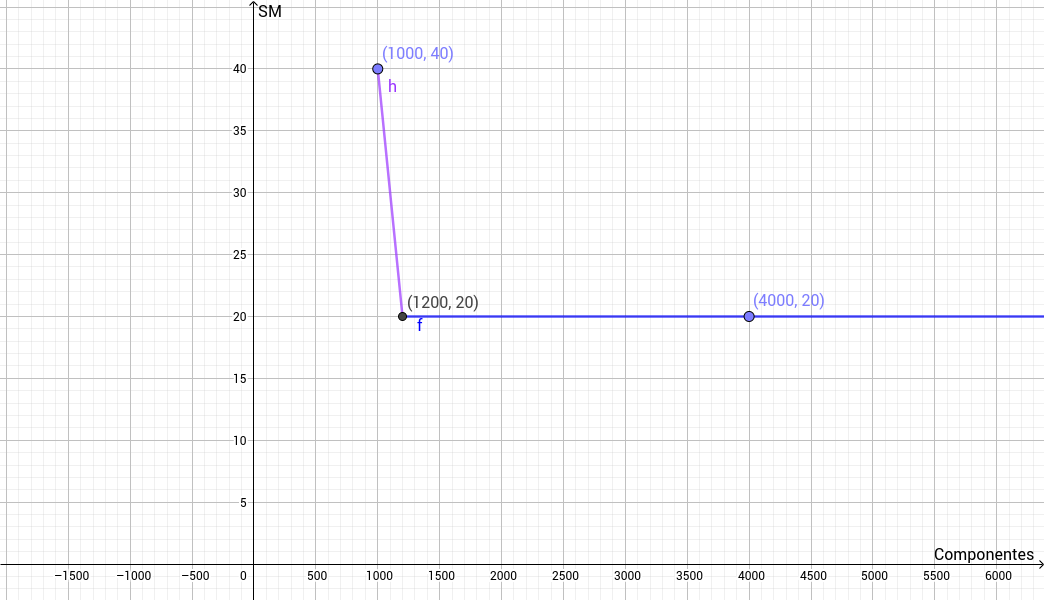
\includegraphics[scale=0.35]{SM.png}
		\end{figure}
		\smallskip
		\begin{figure}[H]
			\caption{Variaci\'on del valor marginal de t\'ecnicos al variar la disponibilidad de componentes.}
			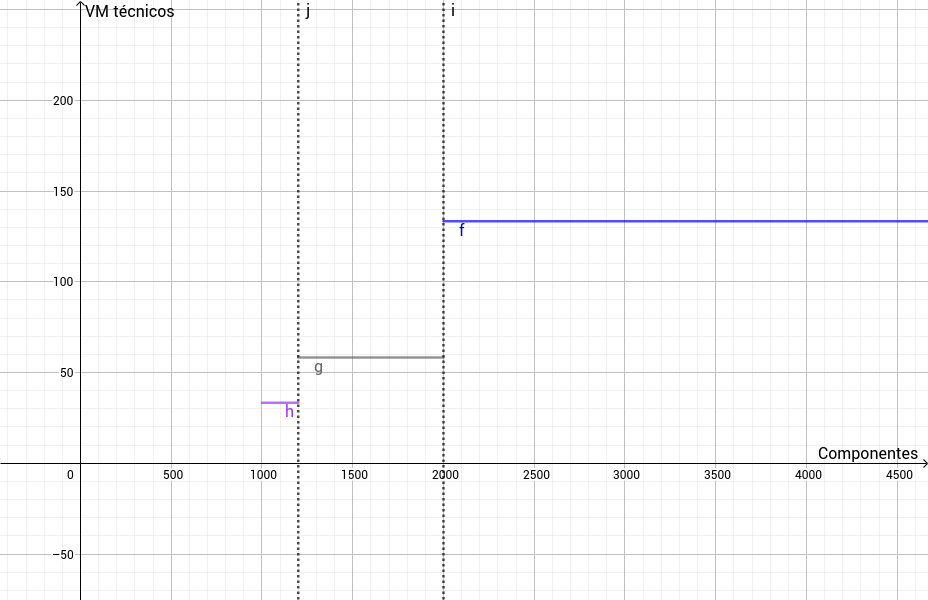
\includegraphics[scale=0.35]{tecncosvm.png}
		\end{figure}
		\smallskip
		\begin{figure}[H]
			\caption{Variaci\'on del funcional al variar la disponibilidad de componentes.}
			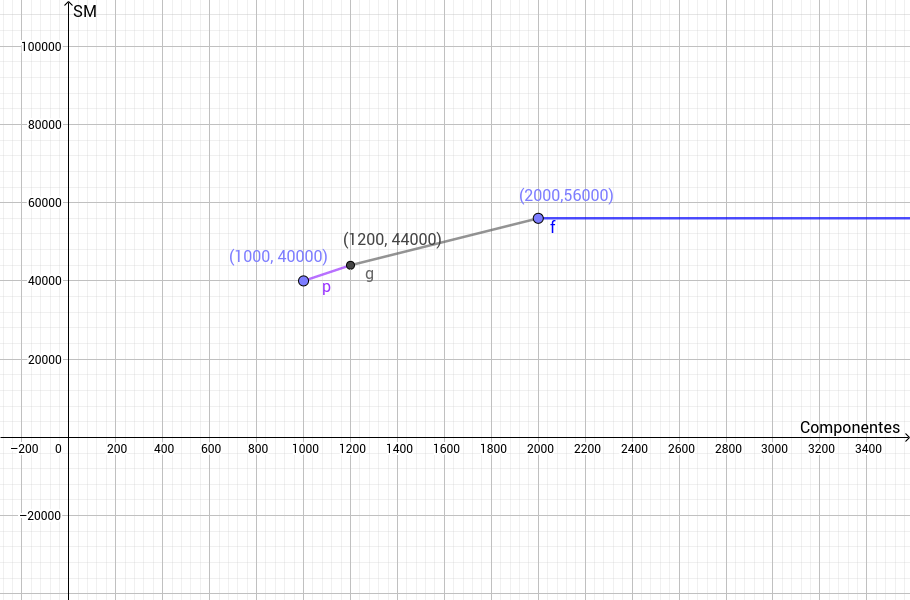
\includegraphics[scale=0.35]{funcional.png}
		\end{figure}
     	\smallskip
	\newpage	
	\item Caso 1:\\
     	\smallskip\\
		\begin{tabular}{|c  c  c | c  c  c  c  c  c  c  c  c | c |}
			\hline
			 \multicolumn{3}{|c|}{} & 3000 & 780 & 120 & -40 & 80 & & & & \\ 
			 Ck & Yk & Bk & A1 & A2 & A3 & A4 & A5 & A6 & A7 & A8 & $\theta$\\ \hline 
			 780 & Y2 & 400/3 & 5 & 1 & 0 & 0 & 0 & -1/3 & 0 & 0 & 400/15\\
			 -40 & Y4 & 200 & 10 & 0 & -1 & 1 & 0 & -1 & 0 & 1 & 20\\
			 0 & Y7 & 150 & 10 & 0 & 0 & 0 & -1 & -1 & 1 & 0 & 15\\ \hline
			 \multicolumn{3}{|c|}{Z=56000} & 500 & 0 & -80 & 0 & -80 & -220 & 0 & -40\\ \hline
		\end{tabular}
		\medskip\\
		Entra Y1, sale Y7\\
		\begin{tabular}{|c  c  c | c  c  c  c  c  c  c  c  c | c |}
			\hline
			 \multicolumn{3}{|c|}{} & 3000 & 780 & 120 & -40 & 80 & & & & \\ 
			 Ck & Yk & Bk & A1 & A2 & A3 & A4 & A5 & A6 & A7 & A8 & $\theta$\\ \hline 
			 780 & Y2 & 175/3 & 0 & 1 & 0 & 0 & 1/2 & 1/6 & -1/2 & 0 & \\
			 -40 & Y4 & 50 & 0 & 0 & -1 & 1 & 1 & 0 & -1 & 1 & \\
			 3000 & Y1 & 15 & 1 & 0 & 0 & 0 & -1/10 & -1/10 & 1/10 & 0 & \\ \hline
			 \multicolumn{3}{|c|}{Z=88500} & 0 & 0 & -30 & 0 & -80 & -170 & -130 & -40\\ \hline
		\end{tabular}
		\medskip\\
		Llegamos a la tabla \'optima.\\
		Ganamos $88500 - 45000 = 43500 < 56000 \Rightarrow $ No conviene.\\
		\smallskip\\
		Caso 2:\\
     	\smallskip\\
		\begin{tabular}{|c  c  c | c  c  c  c  c  c  c  c  c | c |}
			\hline
			 \multicolumn{3}{|c|}{} & 3000 & 80 & 120 & -40 & 80 & & & & \\ 
			 Ck & Yk & Bk & A1 & A2 & A3 & A4 & A5 & A6 & A7 & A8 & $\theta$\\ \hline 
			 80 & Y2 & 400/3 & 5 & 1 & 0 & 0 & 0 & -1/3 & 0 & 0 & 400/15\\
			 -40 & Y4 & 200 & 10 & 0 & -1 & 1 & 0 & -1 & 0 & 1 & 20\\
			 0 & Y7 & 150 & 10 & 0 & 0 & 0 & -1 & -1 & 1 & 0 & 15\\ \hline
			 \multicolumn{3}{|c|}{Z=8000/3 = 2666.6} & -3000 & 0 & -80 & 0 & -80 & 40/3 & 0 & -40 &\\ \hline
		\end{tabular}
		\medskip\\
	    Como el dual tiene soluci\'on \'optima no acotada el primal no tiene soluciones posibles. Por lo tanto este opci\'on tampoco sirve. 
     	\smallskip\\
	    Se puede validar esto dado que no se llegue a proveer la demanda de 40 SM (X3) con solo 40 t\'ecnicos. Se necesitan por lo menos 120 t\'ecnicos para cubrir la demanda.
		\medskip\\

		\newpage
	\item Trabajamos en el primal.\\
     	\smallskip\\
		\begin{tabular}{|c  c  c | c  c  c  c  c  c  c  c  c | c |}
			\hline
			 \multicolumn{3}{|c|}{} & 400 & 450 & 200 & & & & & & \\ 
			 Ck & Xk & Bk & A1 & A2 & A3 & A4 & A5 & A6 & A7 & A8 & $\theta$\\ \hline 
			 400 & X1 & 120 & 1 & 1 & 0 & 0 & 1/3 & 0 & 1 & 0 & 120\\
			 200 & X3 & 40 & 0 & 0 & 1 & 0 & 0 & 0  & -1 & 0 & -\\
			 0 & X4 & 1000 & 0 & -10 & 0 & 1 & -5 & 0 & -10 & 0 & -\\ 
			 0 & X6 & 80   & 0 & 0   & 0 & 0 & 0  & 1 & 1   & 0 & -\\
			 0 & X8 & 80   & 0 & 1   & 0 & 0 & 0  & 0 & 0   & 1 & 80\\ \hline
			 \multicolumn{3}{|c|}{Z=56000} & 0 & -50 & 0 & 0 & 400/3 & 0 & 200 & 0 &\\ \hline
		\end{tabular}
     	\smallskip\\
		\begin{tabular}{|c  c  c | c  c  c  c  c  c  c  c  c | c |}
			\hline
			 \multicolumn{3}{|c|}{} & 400 & 450 & 200 & & & & & & \\ 
			 Ck  & Xk & Bk   & A1 & A2 & A3 & A4 & A5 & A6 & A7 & A8 & $\theta$\\ \hline 
			 400 & X1 & 40  & 1  & 0   & 0 & 0 & 1/3 & 0  & 1   & -1    & \\
			 200 & X3 & 40   & 0  & 0   & 1 & 0 & 0   & 0  & -1  & 0     & \\
			 0   & X4 & 1800 & 0  & 0   & 0 & 1 & -5  & 0  & -10 & 10    & \\ 
			 0   & X6 & 80   & 0  & 0   & 0 & 0 & 0   & 1  & 1   & 0     & \\
			 450   & X2 & 80   & 0  & 1   & 0 & 0 & 0   & 0  & 0   & 1     & \\ \hline
			 \multicolumn{3}{|c|}{Z=60000} & 0 & 0  & 0  & 0   & 400/3 & 0 & 200 & 50 &\\ \hline
		\end{tabular}
     	\smallskip\\
     	
		Llegamos a la tabla \'optima.\\
		El beneficio es de 60000 y se aument\'o la ganancia en 4000 $\Rightarrow$   Conviene.\\
     	
\end{enumerate}
\end{document}
